\documentclass[journal,12pt,twocolumn]{IEEEtran}
%\usepackage{chngcntr}
\usepackage{setspace}
\usepackage{float}
\usepackage{gensymb}
\singlespacing
% \usepackage[cmex10]{amsmath}
\usepackage{caption}
\usepackage{epstopdf}
\usepackage[cmex10]{amsmath}
%\usepackage{amsthm}
%\interdisplaylinepenalty=2500
%\savesymbol{iint}
%\usepackage{txfonts}
%\restoresymbol{TXF}{iint}
%\usepackage{wasysym}
\usepackage{amsthm}
%\usepackage{iithtlc}
\usepackage{mathrsfs}
\usepackage{txfonts}
\usepackage[utf8]{inputenc}
\usepackage{float}
\usepackage{listings}
\usepackage{bm}
\usepackage{mathptmx}
\usepackage{amsfonts}
\usepackage{subfig}
\usepackage{xtab}
\usepackage{longtable}

%\usepackage{algorithm}
%\usepackage{algpseudocode}
%\usepackage{chngcntr}




\usepackage{mathrsfs}
\usepackage{txfonts}
\usepackage{stfloats}
\usepackage{bm}
\usepackage{cite}
% \usepackage{cases}
\usepackage{subfig}

\usepackage{longtable}
% \usepackage{multirow}

\usepackage{enumitem}
\usepackage{mathtools}
% \usepackage{steinmetz}
\usepackage{tikz}
%\usepackage{circuitikz}
\usepackage{verbatim}
% \usepackage{tfrupee}
\usepackage[breaklinks=true]{hyperref}
\usepackage{graphicx}
% \usepackage{tkz-euclide}

\usetikzlibrary{calc,math}
\usepackage{listings}
    \usepackage{color}                                            %%
    \usepackage{array}                                            %%
    \usepackage{longtable}                                        %%
    \usepackage{calc}                                             %%
    %\usepackage{multirow}                                         %%
    \usepackage{hhline}                                           %%
    \usepackage{ifthen}                                           %%
    \usepackage{lscape}     
\usepackage{multicol}
\usepackage{chngcntr}
\usepackage{xcolor}
%\DeclareMathOperator*{\Res}{Res}

\renewcommand\thesection{\arabic{section}}
\renewcommand\thesubsection{\thesection.\arabic{subsection}}
\renewcommand\thesubsubsection{\thesubsection.\arabic{subsubsection}}

\renewcommand\thesectiondis{\arabic{section}}
\renewcommand\thesubsectiondis{\thesectiondis.\arabic{subsection}}
\renewcommand\thesubsubsectiondis{\thesubsectiondis.\arabic{subsubsection}}


\hyphenation{op-tical net-works semi-conduc-tor}
\def\inputGnumericTable{}                                 %%

\lstset{
%language=C,
frame=single, 
breaklines=true,
columns=fullflexible
}
\begin{document}


\newtheorem{theorem}{Theorem}[section]
\newtheorem{problem}{Problem}
\newtheorem{proposition}{Proposition}[section]
\newtheorem{lemma}{Lemma}[section]
\newtheorem{corollary}[theorem]{Corollary}
\newtheorem{example}{Example}[section]
\newtheorem{definition}[problem]{Definition}

\newcommand{\BEQA}{\begin{eqnarray}}
\newcommand{\EEQA}{\end{eqnarray}}
\newcommand{\define}{\stackrel{\triangle}{=}}
\bibliographystyle{IEEEtran}
\raggedbottom
\setlength{\parindent}{0pt}
\providecommand{\mbf}{\mathbf}
\providecommand{\pr}[1]{\ensuremath{\Pr\left(#1\right)}}
\providecommand{\qfunc}[1]{\ensuremath{Q\left(#1\right)}}
\providecommand{\sbrak}[1]{\ensuremath{{}\left[#1\right]}}
\providecommand{\lsbrak}[1]{\ensuremath{{}\left[#1\right.}}
\providecommand{\rsbrak}[1]{\ensuremath{{}\left.#1\right]}}
\providecommand{\brak}[1]{\ensuremath{\left(#1\right)}}
\providecommand{\lbrak}[1]{\ensuremath{\left(#1\right.}}
\providecommand{\rbrak}[1]{\ensuremath{\left.#1\right)}}
\providecommand{\cbrak}[1]{\ensuremath{\left\{#1\right\}}}
\providecommand{\lcbrak}[1]{\ensuremath{\left\{#1\right.}}
\providecommand{\rcbrak}[1]{\ensuremath{\left.#1\right\}}}
\theoremstyle{remark}
\newtheorem{rem}{Remark}
\newcommand{\sgn}{\mathop{\mathrm{sgn}}}
\providecommand{\abs}[1]{\left\vert#1\right\vert}
\providecommand{\res}[1]{\Res\displaylimits_{#1}} 
\providecommand{\norm}[1]{\left\lVert#1\right\rVert}
%\providecommand{\norm}[1]{\lVert#1\rVert}
\providecommand{\mtx}[1]{\mathbf{#1}}
\providecommand{\mean}[1]{E\left[ #1 \right]}
\providecommand{\fourier}{\overset{\mathcal{F}}{ \rightleftharpoons}}
%\providecommand{\hilbert}{\overset{\mathcal{H}}{ \rightleftharpoons}}
\providecommand{\system}{\overset{\mathcal{H}}{ \longleftrightarrow}}
	%\newcommand{\solution}[2]{\textbf{Solution:}{#1}}
\newcommand{\solution}{\noindent \textbf{Solution: }}
\newcommand{\cosec}{\,\text{cosec}\,}
\providecommand{\dec}[2]{\ensuremath{\overset{#1}{\underset{#2}{\gtrless}}}}
\newcommand{\myvec}[1]{\ensuremath{\begin{pmatrix}#1\end{pmatrix}}}
\newcommand{\mydet}[1]{\ensuremath{\begin{vmatrix}#1\end{vmatrix}}}
%\numberwithin{equation}{subsection}

\makeatletter
\@addtoreset{figure}{problem}
\makeatother
\let\StandardTheFigure\thefigure
\let\vec\mathbf

\renewcommand{\thefigure}{\theproblem}

\def\putbox#1#2#3{\makebox[0in][l]{\makebox[#1][l]{}\raisebox{\baselineskip}[0in][0in]{\raisebox{#2}[0in][0in]{#3}}}}
     \def\rightbox#1{\makebox[0in][r]{#1}}
     \def\centbox#1{\makebox[0in]{#1}}
     \def\topbox#1{\raisebox{-\baselineskip}[0in][0in]{#1}}
     \def\midbox#1{\raisebox{-0.5\baselineskip}[0in][0in]{#1}}
\vspace{3cm}
\title{Assignment 1}
\author{G Yashwanth Naik - EE18BTECH11017}
\maketitle
\newpage
\bigskip
\renewcommand{\thefigure}{\theenumi}
\renewcommand{\thetable}{\theenumi}



Download all python codes from 
\begin{lstlisting}
https://github.com/yashwanthguguloth24/EE3025-DSP-lab/tree/main/Assignment1/codes
\end{lstlisting}
%
and latex-tikz codes from 
%
\begin{lstlisting}
https://github.com/yashwanthguguloth24/EE3025-DSP-lab/tree/main/Assignment1
\end{lstlisting}


\section{Problem}
\begin{enumerate}[label=\thesection.\arabic*.,ref=\thesection.\theenumi]
    \numberwithin{equation}{enumi}
    
    \item Let
    \begin{align}
        x(n) = \cbrak{\underset{\uparrow}{1},2,3,4,2,1} \\
        y(n) + \frac{1}{2}y(n-1) = x(n) + x(n-2)	
        \label{eq:equation1}
    \end{align}
    
    \item Compute 
    \begin{align}
        X(k) \triangleq \sum_{n=0}^{N-1} x(n) e^{-j 2 \pi k n / N}, \quad k=0,1, \ldots, N-1
    \end{align}
    and $H(k)$ using h(n).
    
    \item Compute 
    \begin{align}
    Y(k) = X(k)H(k)
    \end{align}

\end{enumerate}

\section{Solution}
\begin{enumerate}[label=\thesection.\arabic*.,ref=\thesection.\theenumi]
\numberwithin{equation}{enumi}
\item
We know that,the Impulse Response of the LTI system is the output of the system when Unit Impulse Signal is given as input to the system.\\
\newline
So, using Eq \eqref{eq:equation1} the Impulse Response of the System can be found as,
\begin{align}
    h(n) + \frac{1}{2}h(n-1) = \delta(n) + \delta(n-2)	
\end{align}
where $h(n)$ is an IIR Filter.
\item DFT of a Input Signal $x(n)$ is 
\begin{align}
    X(k) \triangleq \sum_{n=0}^{N-1} x(n) e^{-j 2 \pi k n / N}, \quad k=0,1, \ldots, N-1
\end{align}
\item DFT of a Impulse Response $h(n)$ is 
\begin{align}
    H(k) \triangleq \sum_{n=0}^{N-1} h(n) e^{-j 2 \pi k n / N}, \quad k=0,1, \ldots, N-1
\end{align}

\item The magnitude and phase plots of $X(k)$ and $H(k)$
\begin{figure}[!ht]
	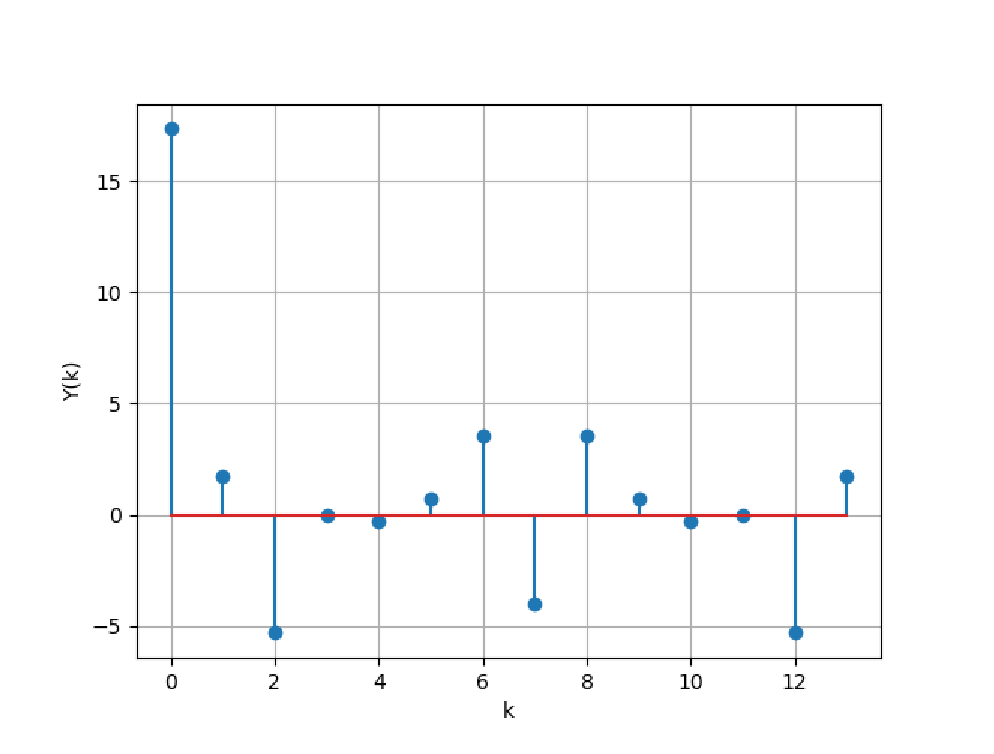
\includegraphics[width=1.15\columnwidth]{./figs/ee18btech11017_fig1.eps}
\end{figure}

\item We can now compute $Y(k)$ using 	Eq \eqref{eq:equation2}

\begin{align}
    Y(k) = X(k)H(k)
    \label{eq:equation2}
\end{align}
The magnitude and phase plots of $Y(k)$ are
\begin{figure}[!ht]
	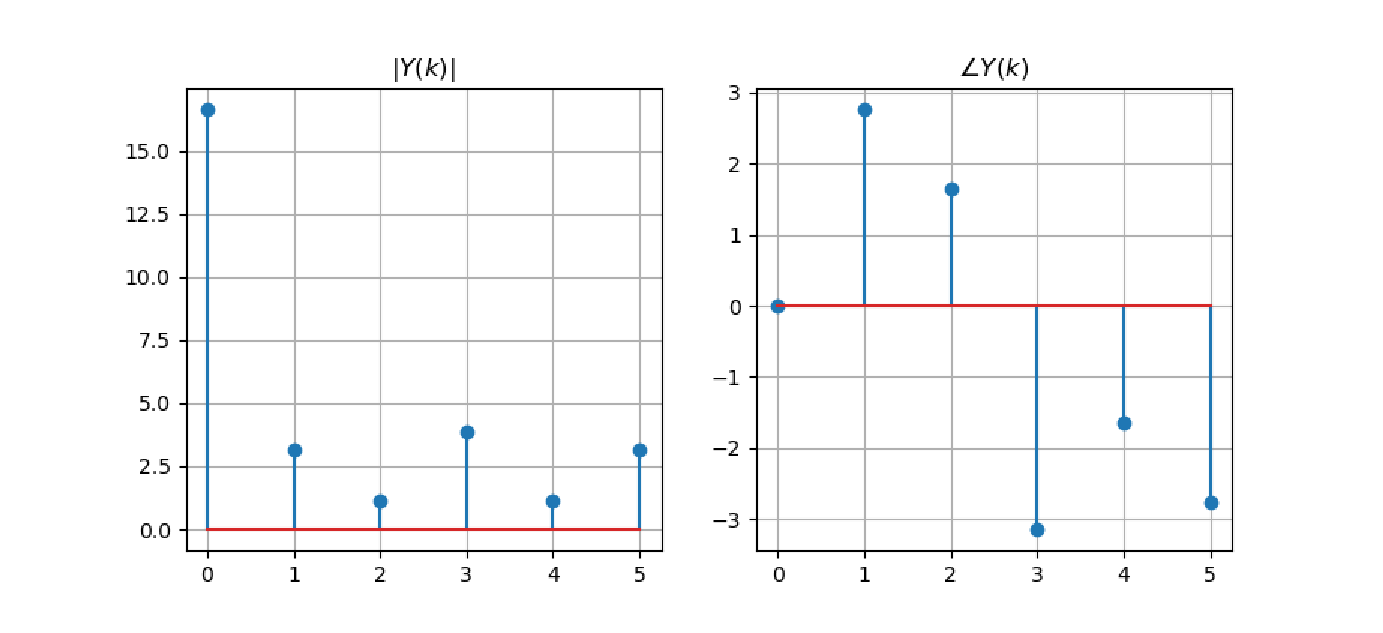
\includegraphics[width=1.15\columnwidth]{./figs/ee18btech11017_fig2.eps}
\end{figure}

\item We can also find $y(n)$ from $Y(k)$ using IDFT formula Eq \eqref{eq:equation3}
\begin{align}
y\brak{n} \triangleq {\frac {1}{N}}\sum _{k=0}^{N-1}Y\brak{k}\cdot e^{j 2\pi kn/N},\quad n = 0,1,\dots, N-1
\label{eq:equation3}
\end{align}

\item The Plot of $y(n)$ using above Eq \eqref{eq:equation3} is
\begin{figure}[!ht]
	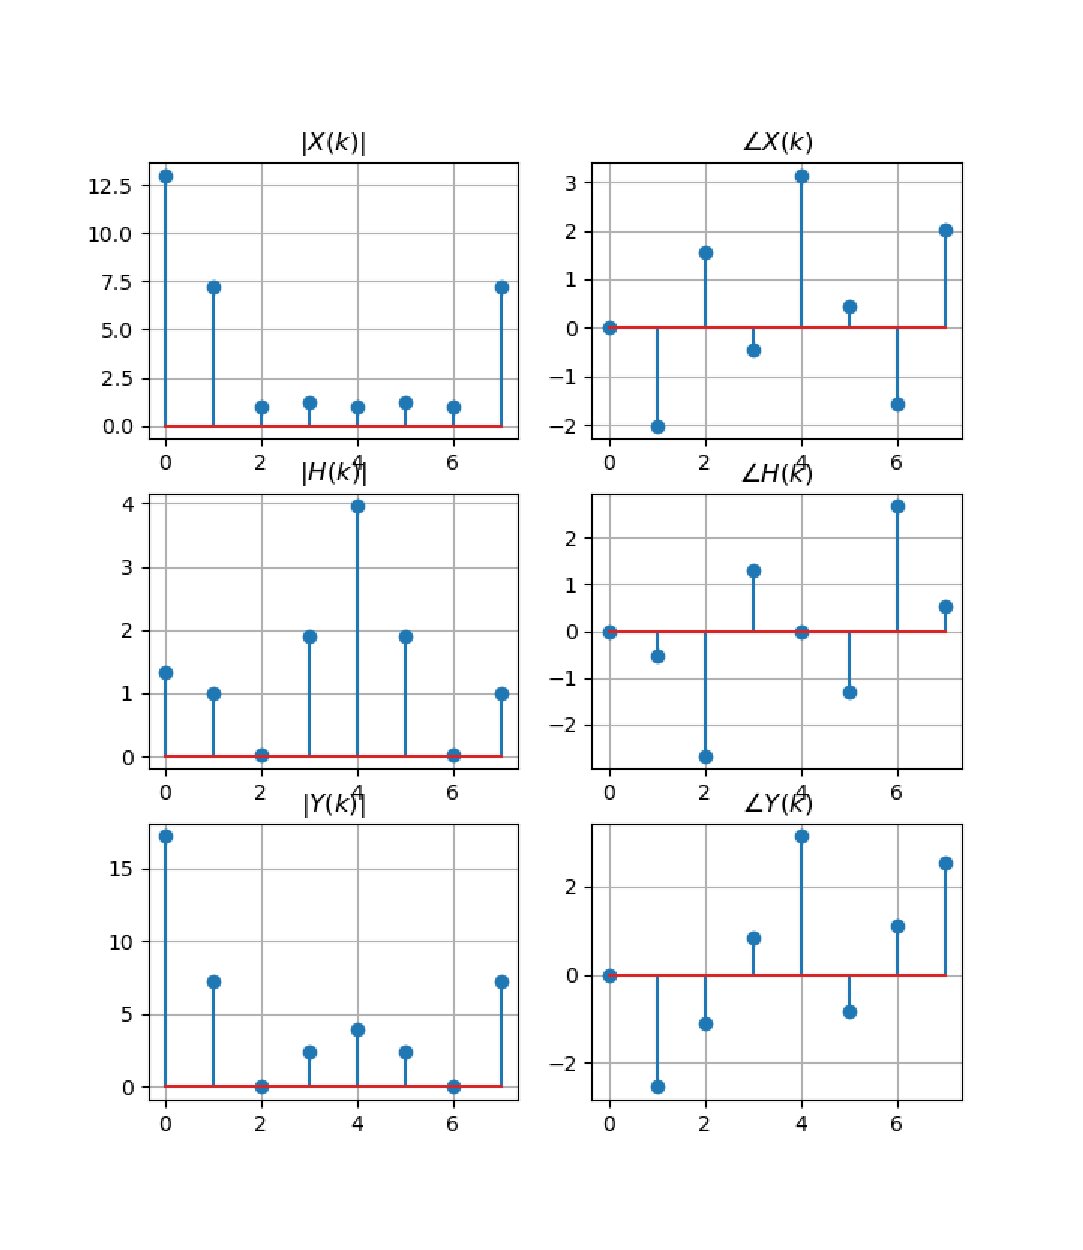
\includegraphics[width=1.15\columnwidth]{./figs/ee18btech11017_fig3.eps}
\end{figure}

\item The following code plots all the above figures.
\begin{lstlisting}
https://github.com/yashwanthguguloth24/EE3025-DSP-lab/tree/main/Assignment1/codes/ee18btech11017.py
\end{lstlisting}

%\item Code for Computing DFT of $x(n)$ and $h(n)$
%\solution\\
%Assuming length of $h(n)$ is $250$ for better plotting of Frequency Components.\\
%\newline
%Code is in
%\begin{lstlisting}
%    codes/ee18btech11017.py
%\end{lstlisting}
%Magnitude and Phase Plots of $X(k)$ and $H(k)$

\end{enumerate}


























\end{document}
